% Please read README.md on how to edit, deliver, or change the documentation

\documentclass[letterpaper,12pt]{article}
\usepackage{graphicx}
\usepackage{tabularx}
\usepackage{listings}
\usepackage{hyperref}

% Hide outline and color of URL and Table of Contents links
\hypersetup{hidelinks}

% Location of image resources
\graphicspath{ {./documentation/res/} }

% Document information

\title{Water Weather Stations Documentation}
\author{
  Grant Barton \and
  Jacob DeBoer  \and
  Karina Sandlin \and
  Ryan Lingg \and
  Sara Morimoto \and
  Daniel Shtunyuk \and
  Elana Cueto \and
  Erik Fretheim \and
  Harry Saliba \and
  Morgan Stimpson \and
  Paul Haithcock \and
  Vipul Kumar \and
  Alex Wilson \and
  Jay Hechter \and
  Douglas Woods \and
  Jessica Avery
}

\begin{document}
  \maketitle
  \newpage
  \tableofcontents
  \newpage
  % Introduction to the project and this document, elements taken from the most recent Vision and Scope
  \section{Introduction}
  % State the purpose of this document
  \subsection{Purpose}
  \textbf{This document is not designed to be given to students.} It is for instructors and camp directors to reference to create a curriculum for students. You will find information on how the systems work in detail, and how to diagnose and correct issues. It is recommended that an instructor reads sections of this document such as buoy construction, buoy operation, android app operation, and web app operation.  Then, create a curriculum for the group of students they are instructing based on the material.
  % Background of the Water Weather Station
  \subsection{Background}
  The Weather Water Stations project is an ongoing project with the SEA Discovery Center located in Paulsbo, WA. The projects goal is to educate youth campers on cyber-security, computer science, and electrical engineering. Students take a camp at the SEA Discovery Center and are able to take home a Water Weather Station in a small form factor to take readings of multiple water conditions.
  % Answer, what is to gain from the use of the Water Weather Stations? No need to go into detail about users and actors, this is most likely not going to be read by a CS Major
  \subsection{Opportunity}
  The project offers an educational tool for students that will attend the camp at the SEA Discovery Center. This will give youth an opportunity to learn more about how a system involving hardware, networking, and security to capture sensor data to create meaningful information about the current water conditions. This information is valuable, as it can be used to analyze changes in water conditions in many areas across the region.
  % Pull in external documentation files
  % This document is designed as a very basic user guide for how to use the Water Weather Station, additional information can be found in the operation manual for each section of this project
\section{Basic User Guide}
% Very brief purpose statement for the user guide
The WWXS offers a unique way of keeping students engaged beyond the end of their camp. The buoy will allow for physical interaction with a device that creates useful data. With a higher level of user interaction students will be more likely to retain the skills they have learned at the Sea Discovery Camp. This user guide will give a brief operation overview of the entire system.
\subsection{The Buoy}
% Quick description of the physical device, include an image.

% see more in device operation
Read more in section \ref{device-operation}
\subsection{Android App}
% Quick description of the android application, how it connects to the device (if you were explaining it to a non-cs-person).

% see more in android app operation
Read more in section \ref{android-app-operation}
\subsection{Website}
% Quick description of what the website does and why we have it.

% see more in web app operation
Read more in section \ref{web-app-operation}
  % This document should describe, in detail, how to use the device
\section{Device Operation} \label{device-operation}

\subsection{Bluetooth Commands}

\begin{flushleft}
    The ESP32 responds to 2 specific Bluetooth LE GATT commands, a Control characteristic and a Data characteristic.
\end{flushleft}

\begin{center}
    \begin{tabular}{ |l|l|l|l| }
        \hline 
        \footnotesize Characteristic & \footnotesize UUID & \footnotesize Value Handle & \footnotesize Permissions \\
        \hline 
        \scriptsize Control & \scriptsize 0000abc0-0000-1000-8000-00805f9b34fb & \scriptsize 0x002a & \scriptsize R, W \\
        \hline 
        \scriptsize Data & \scriptsize 0000abc1-0000-1000-8000-00805f9b34fb & \scriptsize 0x002d & \scriptsize R, W, N \\
        \hline
    \end{tabular}
\end{center}

\subsubsection{Station Start - Sequence diagram}

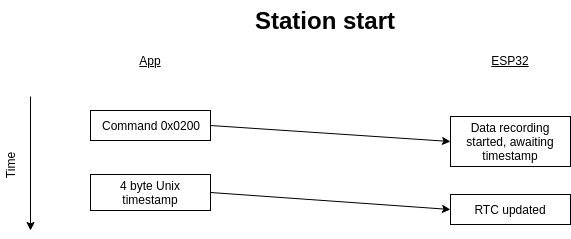
\includegraphics[scale=0.63]{buoy-rtc.png}

\subsubsection{Data Collection - Sequence diagram}

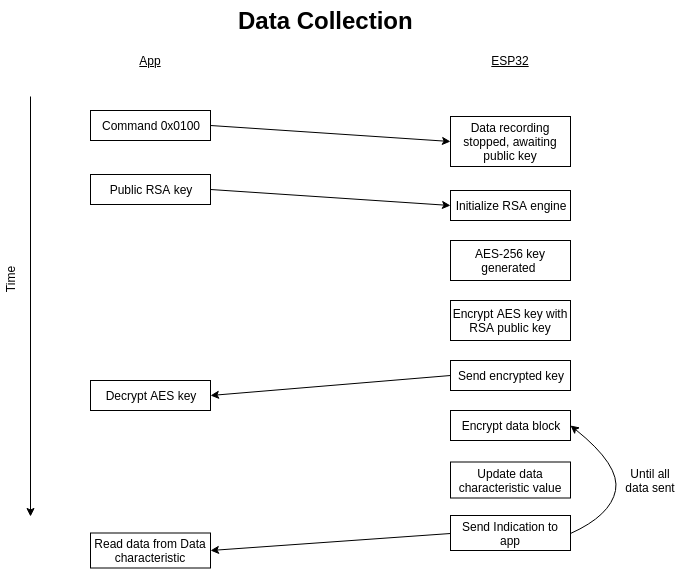
\includegraphics[scale=0.63]{buoy-data.png}

\subsection{Powering On and Connecting to the buoy}

When protoypting, connecting the Micro USB cable to the ESP32 development board to power up the device with 5 volts.
When using the production buoy, make sure 2 AA batteries are in the battery pack. Switch the power switch to ON.
Once the buoy is receiving power, it will boot up and initialize the Bluetooth Low-Energy after which the Android app may connect to the buoy through Bluetooth.
  % Describe, in detail, how to use the android app
\section{Android App Operation} \label{android-app-operation}
  % Describe how to use the website
\section{Web App Operation} \label{web-app-operation}
  % This document should list all the parts for the device
\section{Parts List}

\subsection{Part quantities}

\begin{tabular}{|l|c|}
    \hline
    \textbf{Part} & \textbf{Qty.}\\
    \hline
    \hyperlink{esp32}{SparkFun ESP32 Thing} & 1\\
    \hline
    \hyperlink{light}{Photoresistor GM5539} & 1\\
    \hline
    \hyperlink{temp}{Temperature Sensor} & 3\\
    \hline
    \hyperlink{salinity}{Water Sensor} & 1\\
    \hline
    \hyperlink{turbidity}{Turbidity Sensor} & 1\\
    \hline
    \hyperlink{nalgene}{Nalgene Bottle} & 1\\
    \hline
    \hyperlink{cable}{2-ft. Waterproof cable} & 1\\
    \hline
    \hyperlink{cable}{6-ft. Waterproof cable} & 1\\
    \hline
    \hyperlink{minibread}{Mini Breadboard} & 2\\
    \hline
    \hyperlink{jumperwires}{M-to-M jumper wires} & 2\\
    \hline
    \hyperlink{jumperwires}{M-to-F jumper wires} & 14\\
    \hline
    \hyperlink{jumperwires}{F-to-F jumper wires} & 2\\
    \hline
    \hyperlink{batteryholder}{2-AA battery holder} & 1\\
    \hline
    \hyperlink{battery}{AA battery} & 2\\
    \hline
    \hyperlink{silica}{Silica gel packet} & 2\\
    \hline
    \hyperlink{glue}{Silicone glue} & 1\\
    \hline

\end{tabular}

% Each subsection is a category of parts
\subsection{System on a chip (SoC)}

% first, name of item
\hypertarget{esp32}{}
\subsubsection{SparkFun ESP32 Thing}

% second, image
\hspace{2em}
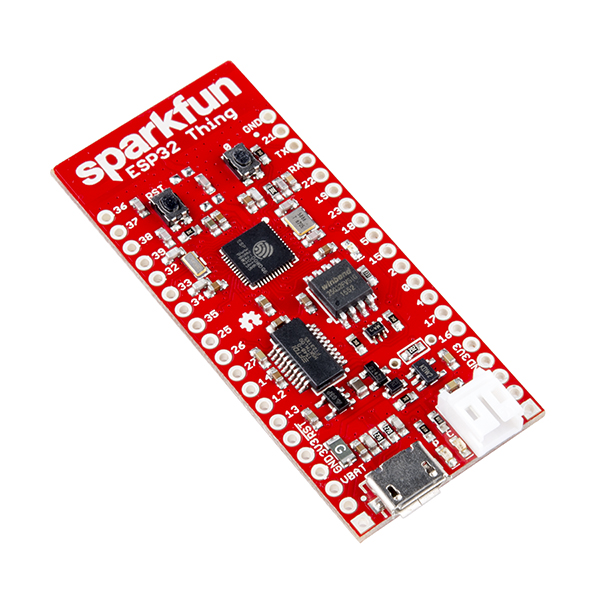
\includegraphics[scale=1.0]{esp32Soc.jpg}

\begin{flushleft}
% third, short description
    The main processing unit is a SparkFun ESP32 Thing development board from 
    Espressif. This SoC has Wi-Fi, Bluetooth 4.0, and BLE capabilities, which 
    are necessary for our system.
    \newline

    % fourth, store link
    Online store link: \newline
    \footnotesize\url{https://www.sparkfun.com/products/13907}

    % fifth, data-sheet link
    \normalsize Datasheet link: \newline
    \footnotesize\url{https://cdn.sparkfun.com/datasheets/IoT/esp32_datasheet_en.pdf}
\end{flushleft}

\subsection{Sensors}

\hypertarget{light}{}
\subsubsection{Photoresistor GM5539}

\hspace{2em}
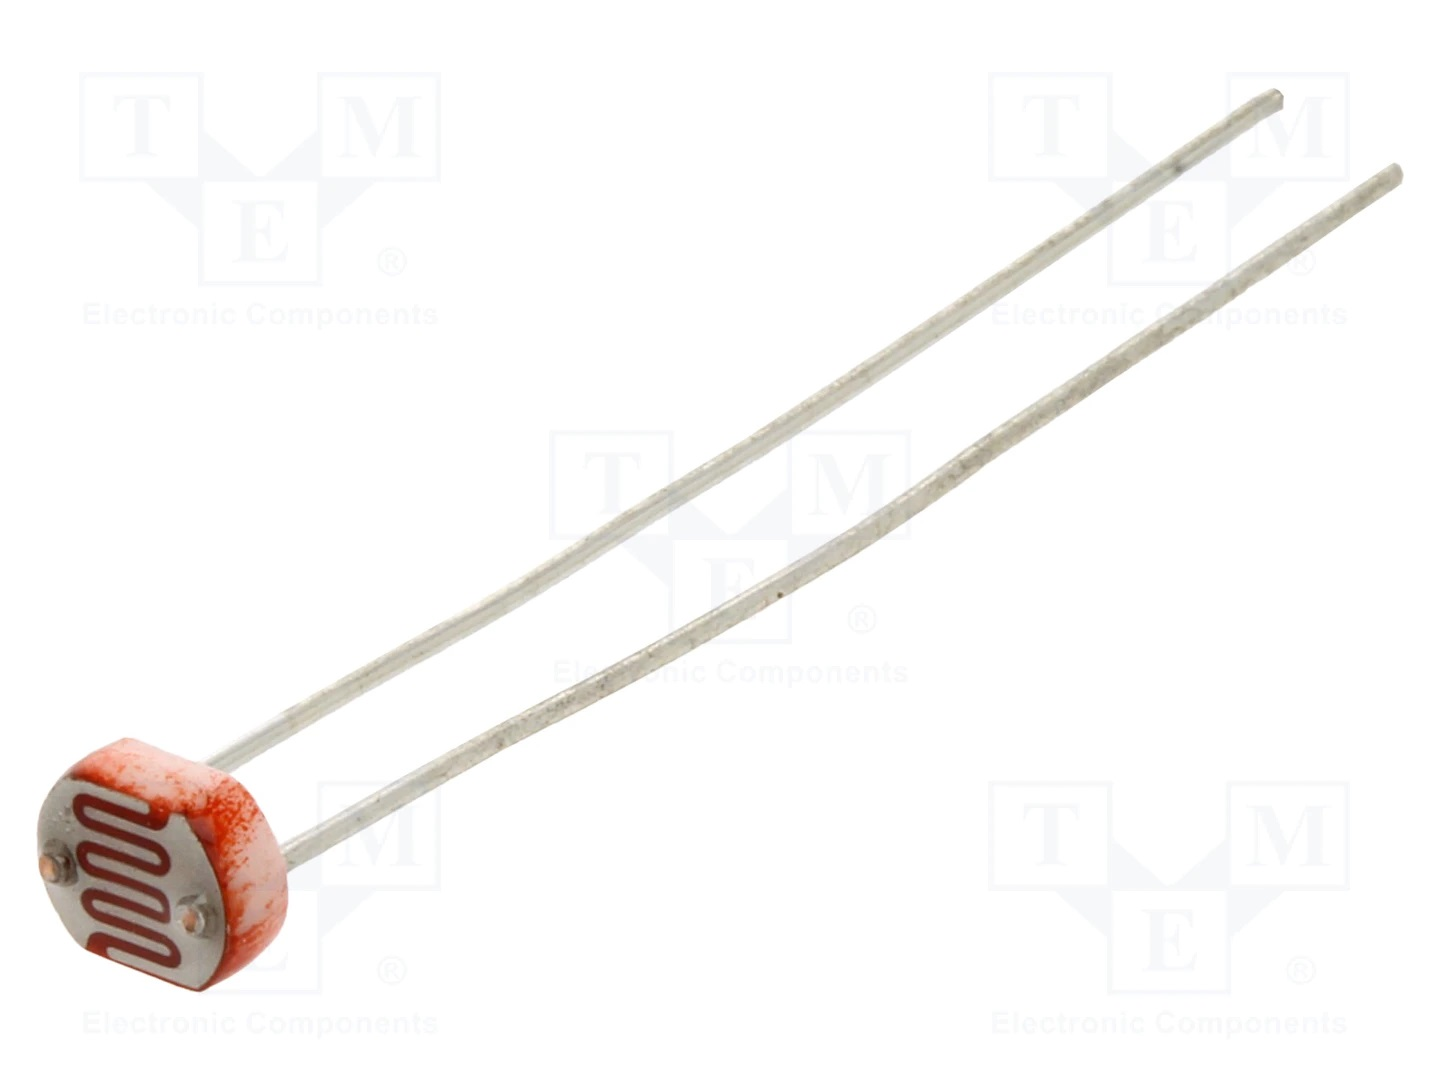
\includegraphics[scale=0.15]{photoresistor.jpg}

\begin{flushleft}
    The GM5539 Photoresistor is used to measure the amount of light hitting the
     sensor.
    \newline

    Online store link: \newline
    \footnotesize\url{https://www.amazon.com/goeasybuy-Sensitive-Resistor-Photoresistor-Optoresistor/dp/B01CGCNO34}

    \normalsize Datasheet link: \newline
    \footnotesize\url{https://www.tme.eu/Document/01ba1573cea1124ddd9a55cccc53ed63/all.pdf}
\end{flushleft}

\hypertarget{temp}{}
\subsubsection{Temperature Sensor}

\hspace{2em}
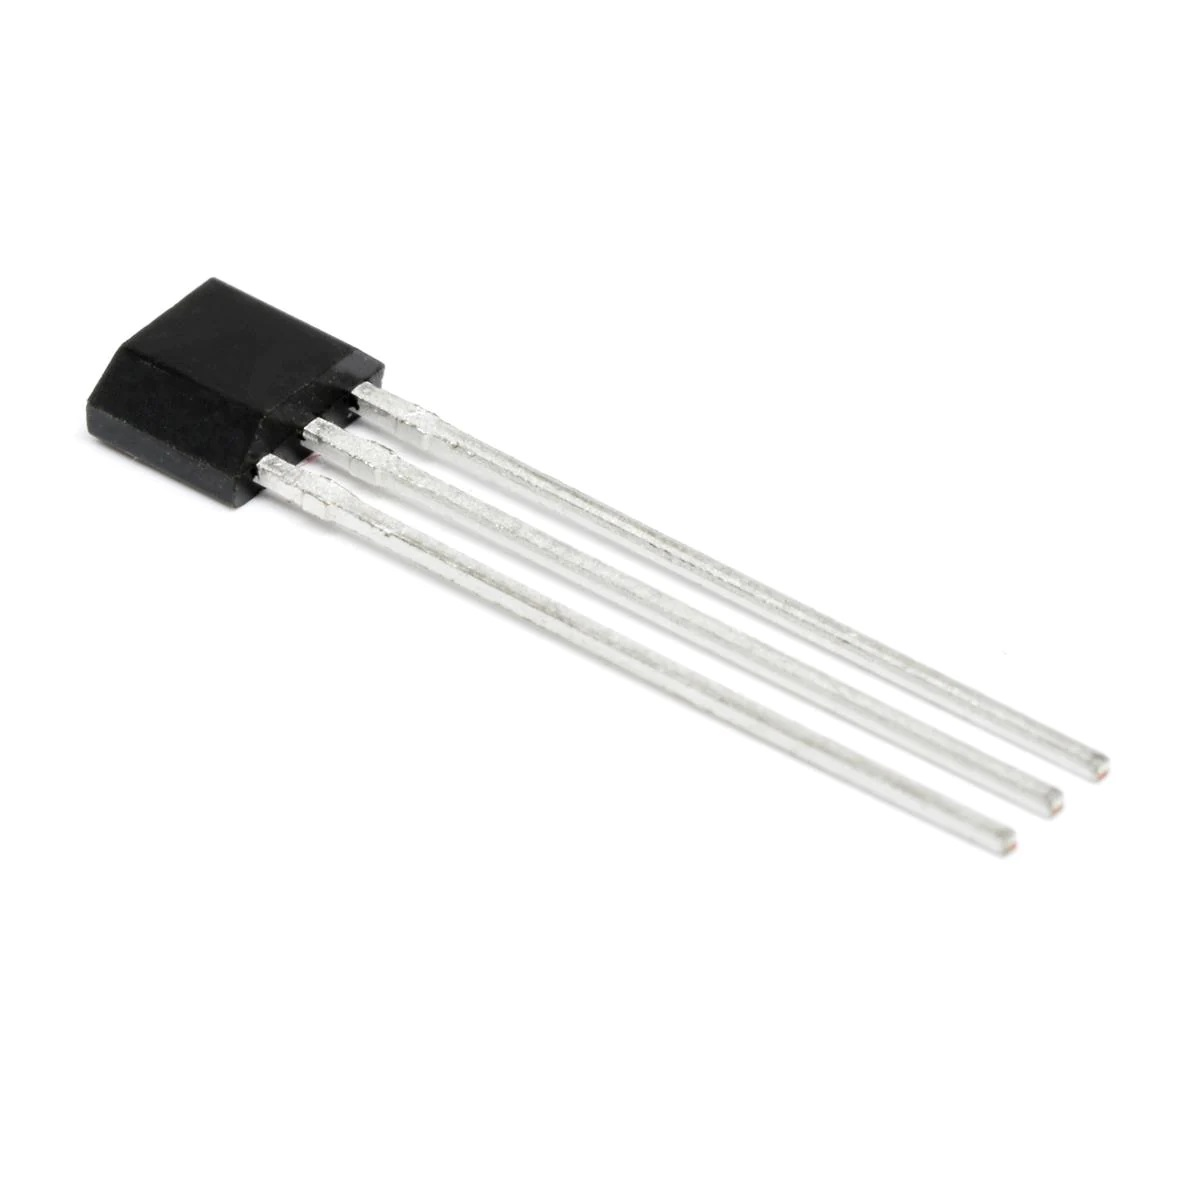
\includegraphics[scale=0.15]{tempsensor.jpg}

\begin{flushleft}
    The TMP36GT9Z temperature sensor from Analog Devices is used to measure 
    the temperature inside the nalgene bottle (at the surface level), 
    immediately underneath the water by the nalgene bottle, and 6 feet deep in 
    the water.
    \newline

    Online store link: \newline
    \footnotesize\url{https://www.mouser.com/ProductDetail/Analog-Devices/TMP36GT9Z?qs=sGAEpiMZZMv9Q1JI0Mo%2FtZYNPIqRJ81F}

    \normalsize Datasheet link: \newline
    \footnotesize\url{https://www.mouser.com/datasheet/2/609/TMP35_36_37-1504323.pdf}
\end{flushleft}

\hypertarget{salinity}{}
\subsubsection{Water Sensor}

\hspace{2em}
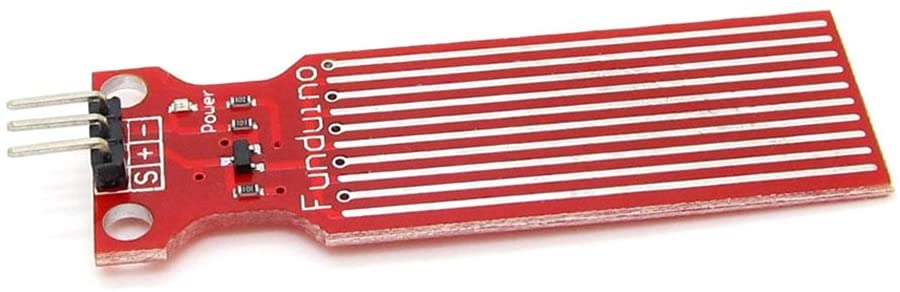
\includegraphics[scale=0.2]{watersensor.jpg}

\begin{flushleft}
    The water sensor is to detect the salinity of the water. Purely diststilled
     water will not be detected, but the contacts will corrode more as it stays
     longer in the water with the more salinity in the water. The more salinity
     that is in contact, the more energy is flowed through the contacts.
    \newline

    Online store link: \newline
    \footnotesize\url{https://www.amazon.com/Sensor-module-Detection-Surface-Arduino/dp/B01N058HS6/}

    \normalsize Datasheet link: \newline
    \footnotesize \emph{N/A}
\end{flushleft}

\hypertarget{turbidity}{}
\subsubsection{Turbidity Sensor}

\hspace{2em}
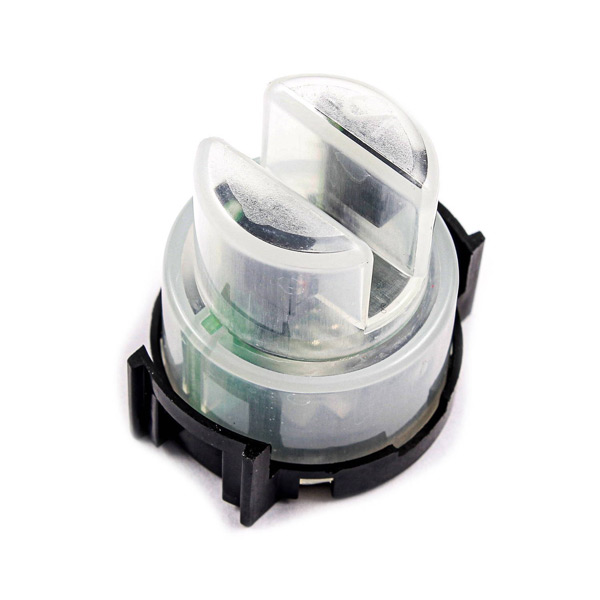
\includegraphics[scale=0.15]{turbidity.jpg}

\begin{flushleft}
    The TSD-10 turbidity sensor from Amphenol Advanced Sensors is to measure 
    the amount of light being received from the output source to the sensor.
    \newline

    Online store link: \newline
    \footnotesize\url{https://www.newark.com/amphenoladvanced-sensors/tsd-10/turbidity-sensor-5vdc-phototransistor/dp/18X9859}

    \normalsize Datasheet link: \newline
    \footnotesize\url{http://www.farnell.com/datasheets/1855958.pdf}
\end{flushleft}

\subsection{Prototyping/Development}

\subsubsection{Breadboard}

\hspace{2em}
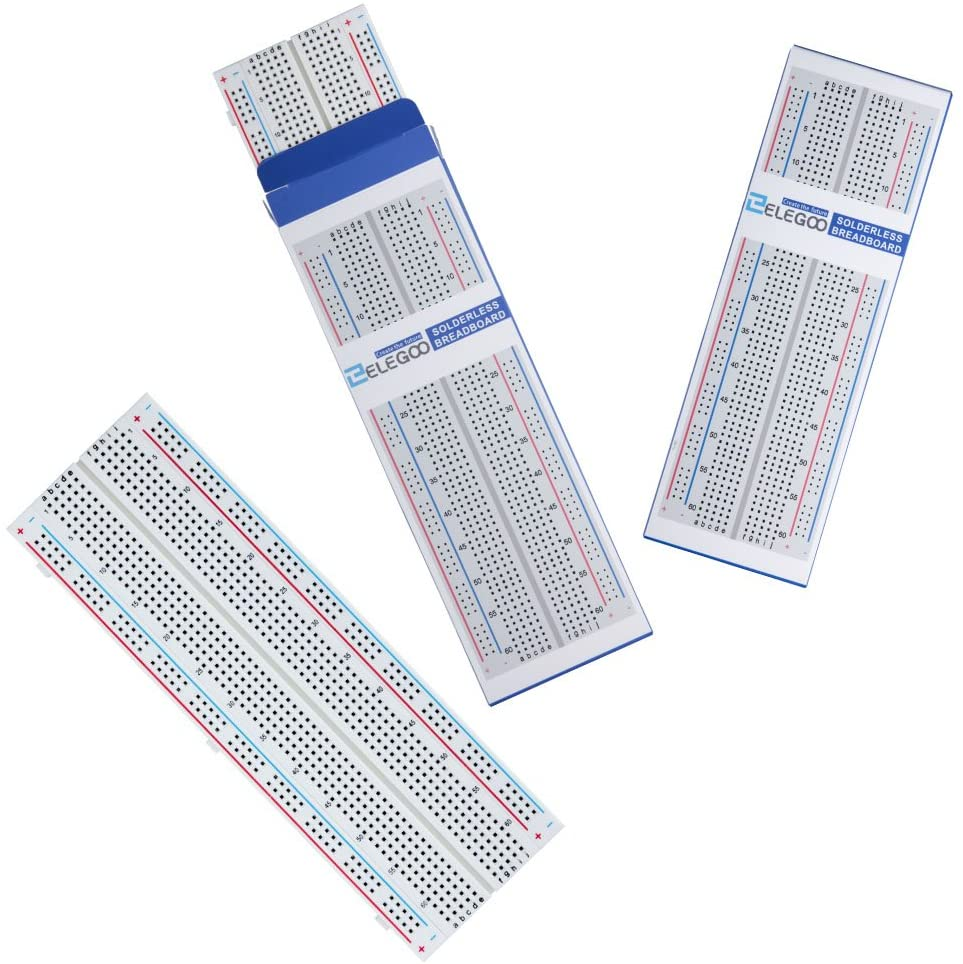
\includegraphics[scale=0.1]{breadboard.jpg}

\begin{flushleft}
    A simple yet useful platform to easily design and prototype circuits for 
    the hardware buoy. Keeps everything attached to one platform, like the 
    sensors, SoC, and wiring.
    \newline

    Online store link: \newline
    \footnotesize\url{https://www.amazon.com/EL-CP-003-Breadboard-Solderless-Distribution-Connecting/dp/B01EV6LJ7G}

\end{flushleft}

\subsubsection{Breadboard wires}

\hspace{2em}
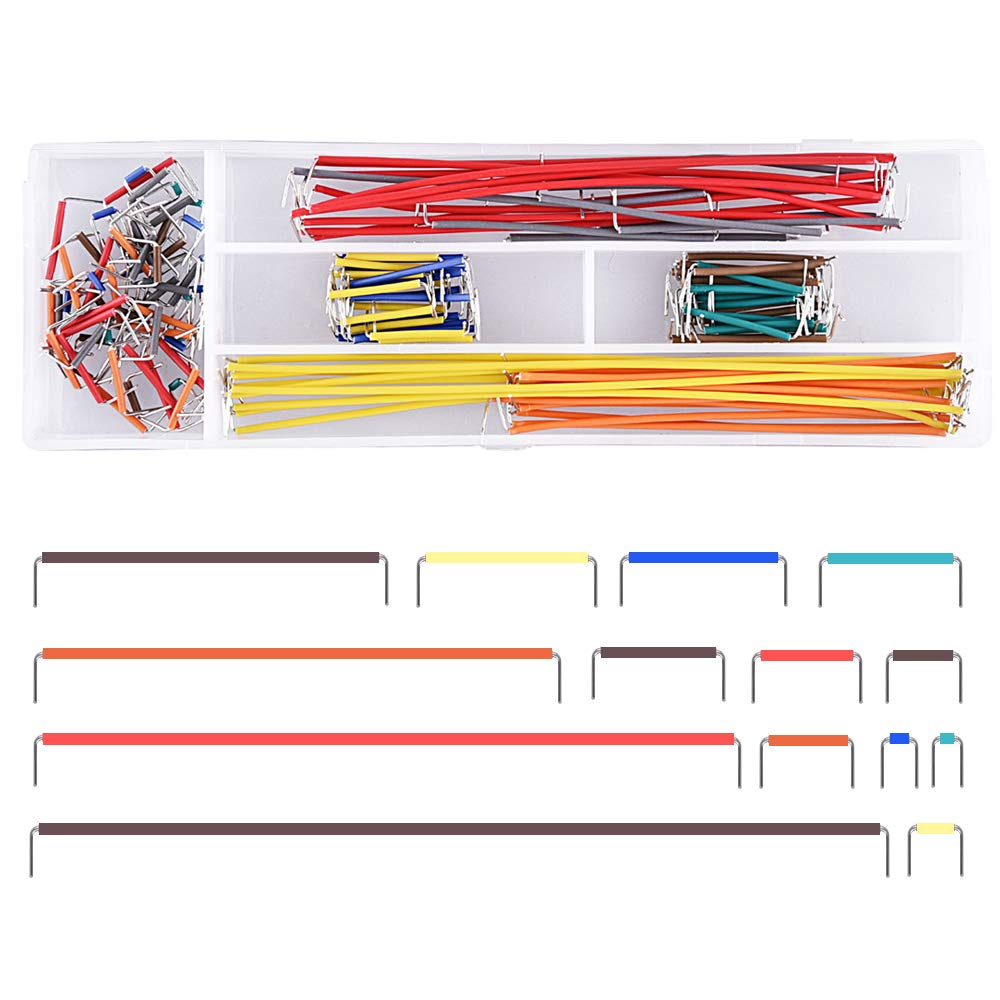
\includegraphics[scale=0.07]{breadboardwires.jpg}

\begin{flushleft}
    Layout the circuit with various sized wires to make a clean and modifiable 
    design for the hardware buoy.
    \newline

    Online store link: \newline
    \footnotesize\url{https://www.amazon.com/AUSTOR-Preformed-Breadboard-Assorted-Prototyping/dp/B07PQKNQ22}

\end{flushleft}

\subsection{Production Buoy}

\hypertarget{nalgene}{}
\subsubsection{Nalgene Bottle}

\hspace{2em}
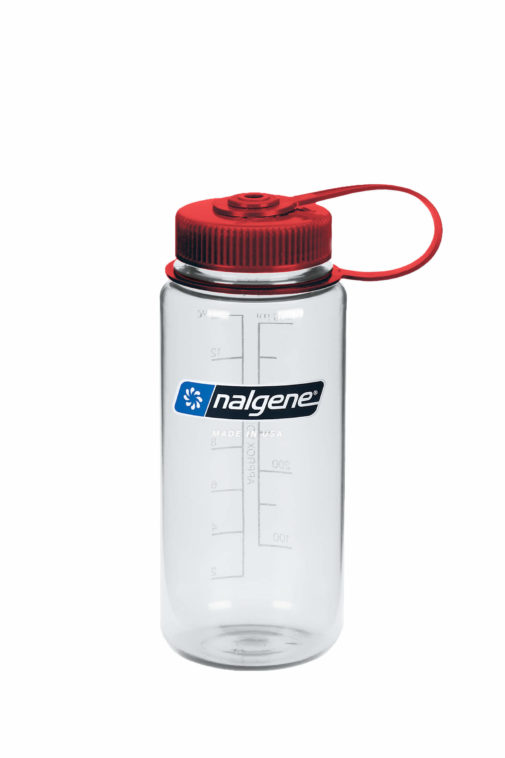
\includegraphics[scale=0.12]{nalgene.jpg}

\begin{flushleft}
    16 oz. Nalgene bottle featuring a screw-top lid for the mouth opening. 
    This is the vessel for our hardware, which will live inside the bottle 
    with 2 outlets (holes) that will be made in the lid to lead out sensors 
    out to 2 feet and 6 feet underneath the water.
    \newline

    Online store link: \newline
    \footnotesize\url{https://nalgene.com/product/16oz-wide-mouth-bottle/?attribute_pa_color=clear}

\end{flushleft}

\hypertarget{cable}{}
\subsubsection{Waterproof cable}

\hspace{2em}
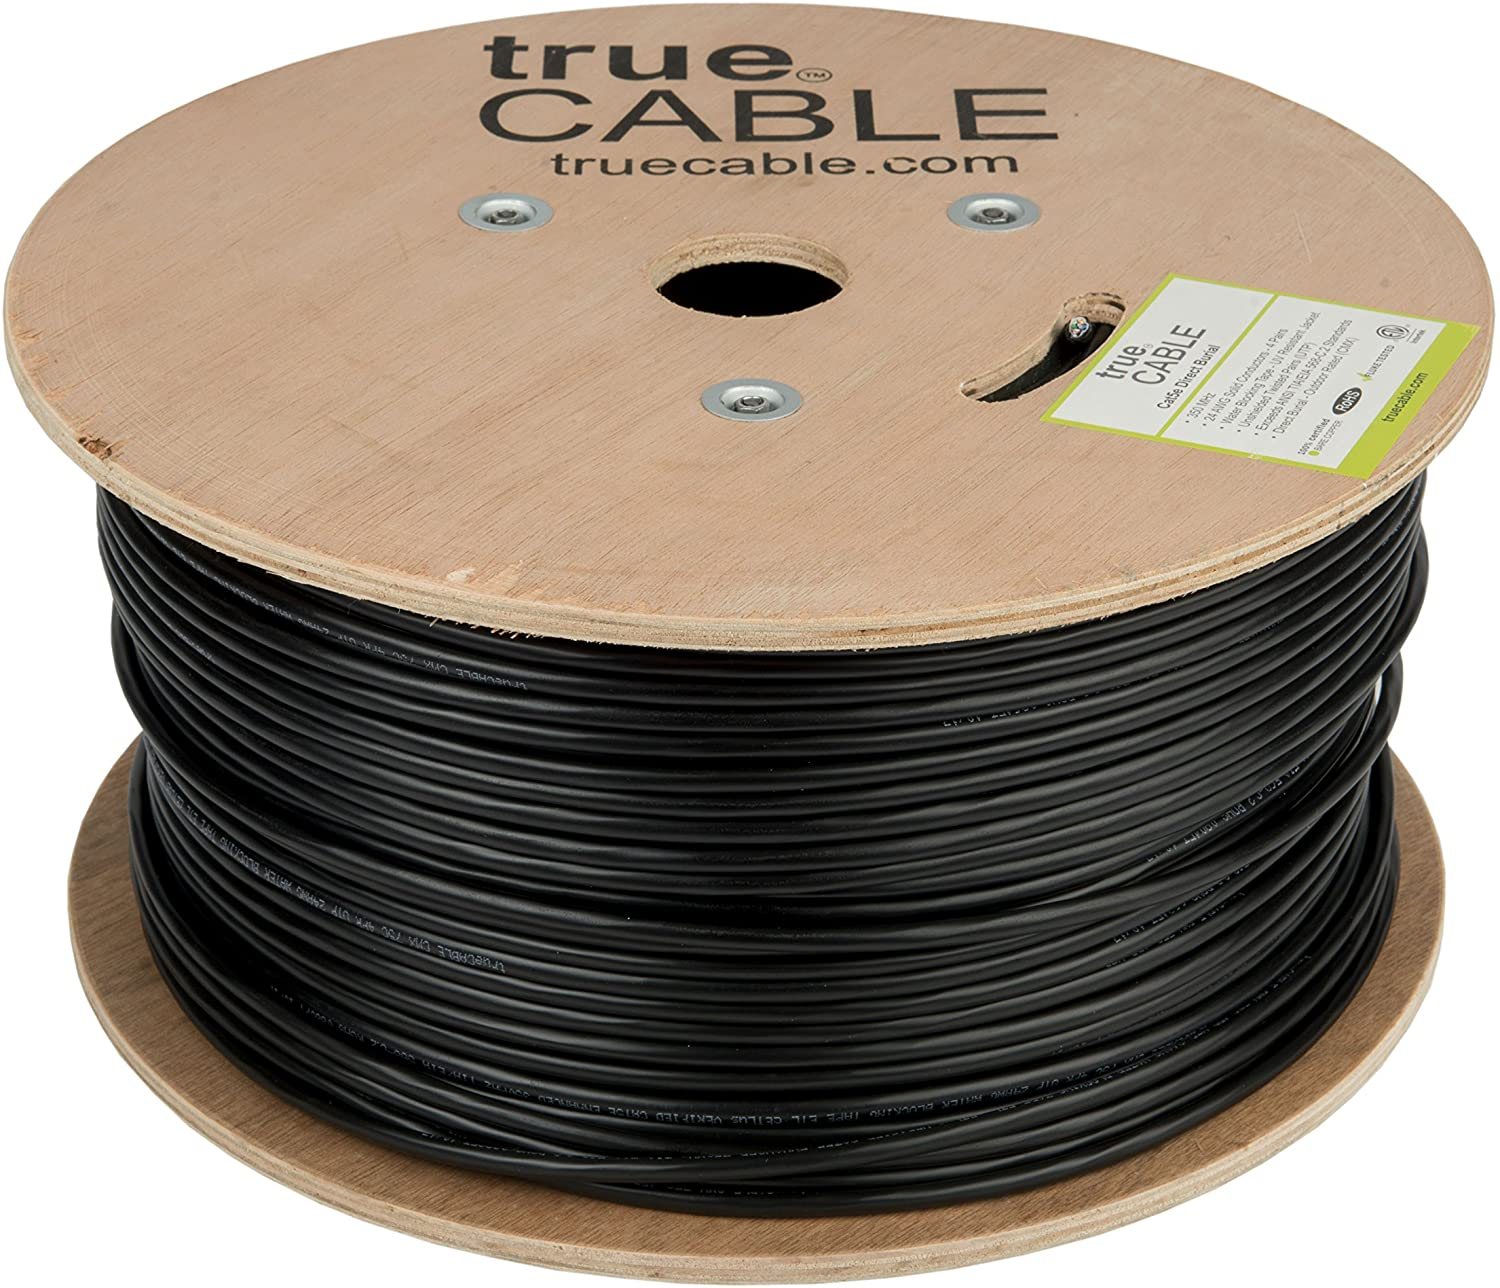
\includegraphics[scale=0.08]{ethernetcable.jpg}

\begin{flushleft}
    This Cat5e cable has a waterproof rating, which is perfect for our 
    application. There are many leads available to wire up all the sensors to 
    the ESP32. This cord will be cut into a 2-foot piece and a 6-foot piece.
    It comes in a 500-foot roll.
    \newline

    Online store link: \newline
    \footnotesize\url{https://www.amazon.com/dp/B01JAVNK2E}

\end{flushleft}

\hypertarget{minibread}{}
\subsubsection{Mini Breadboard}

\hspace{2em}
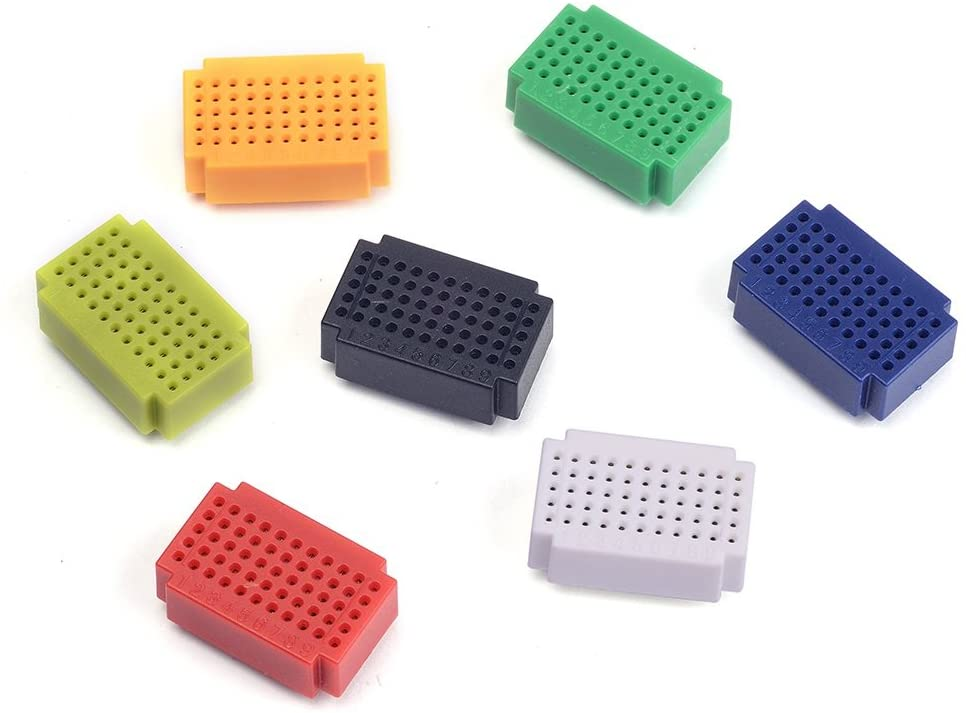
\includegraphics[scale=0.1]{minibreadboard.jpg}

\begin{flushleft}
    Smaller, more managable breadboard in a tight volume of the nalgene bottle 
    will help keep all the wiring together and provide power for all sensors.
    \newline

    Online store link: \newline
    \footnotesize\url{https://www.amazon.com/Cylewet-Solderless-Circuit-Arduino-CYT1030/dp/B01N9MIH1T}

\end{flushleft}

\hypertarget{jumperwires}{}
\subsubsection{Jumper wires}

\hspace{2em}
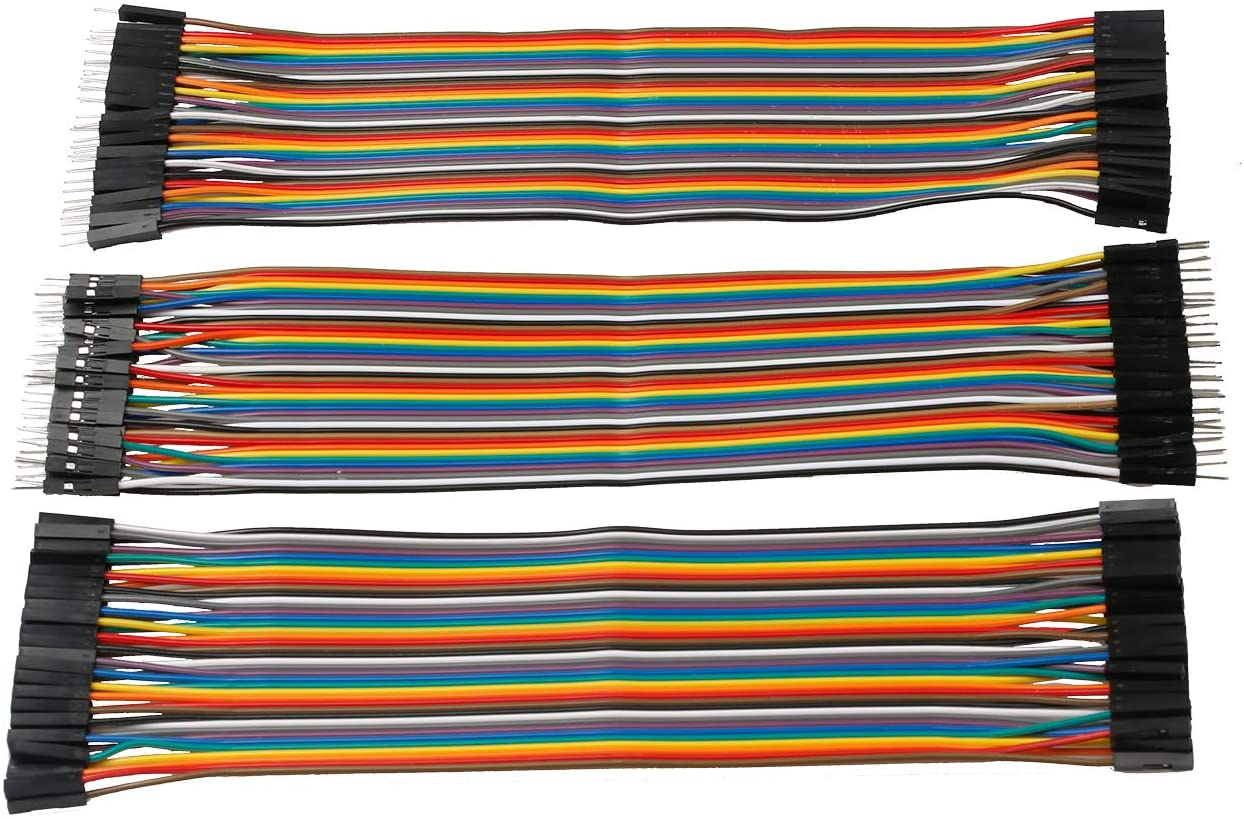
\includegraphics[scale=0.1]{jumperwires.jpg}

\begin{flushleft}
    A set of Male-to-Male, Male-to-Female, and Female-to-Female breadboard 
    jumper wires for connecting the photoresistor, temperature, and ESP32 pins 
    together to the breadboards. Each buoy only needs about 12 wires, but the 
    linked set of jumper wires offers the best price.
    \newline

    Online store link: \newline
    \footnotesize\url{https://www.amazon.com/EDGELEC-Breadboard-Optional-Assorted-Multicolored/dp/B07GD2BWPY/}

\end{flushleft}

\hypertarget{batteryholder}{}
\subsubsection{2-AA battery holder}

\hspace{2em}
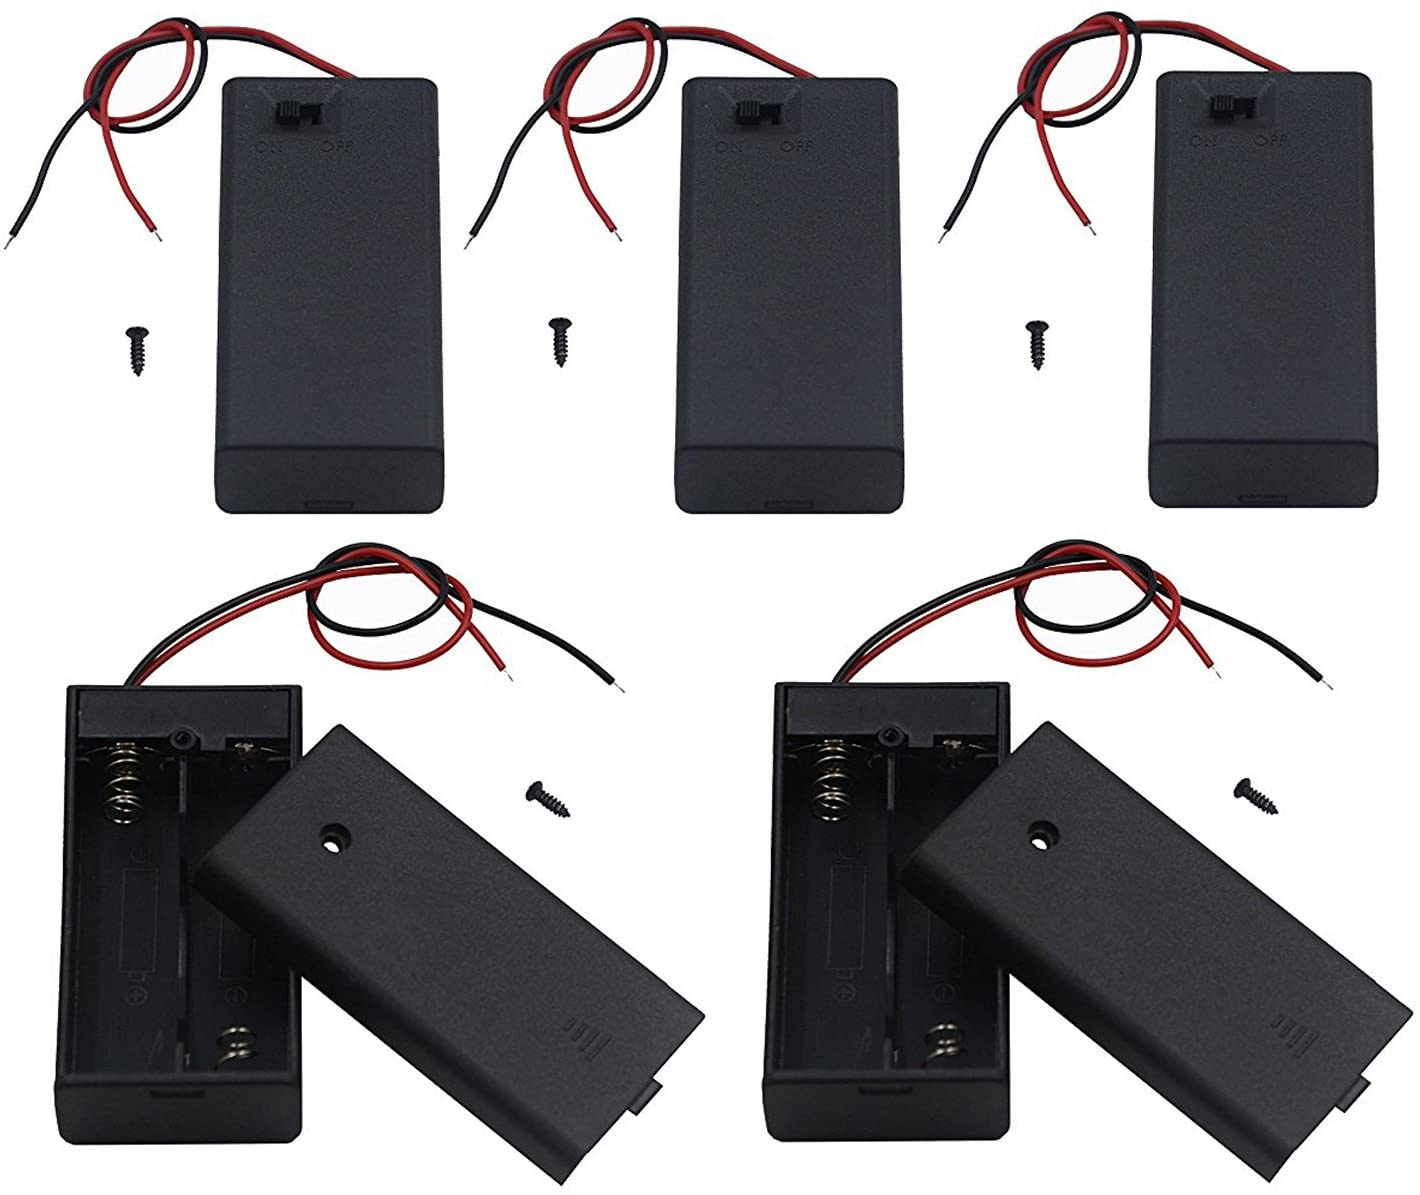
\includegraphics[scale=0.1]{batteryholder.jpg}

\begin{flushleft}
    An AA battery holder with positive and negative lead wires and a 
    power switch.
    \newline

    Online store link: \newline
    \footnotesize\url{https://www.amazon.com/dp/B076C7S2VN/}

\end{flushleft}

\hypertarget{battery}{}
\subsubsection{AA batteries}

\hspace{2em}
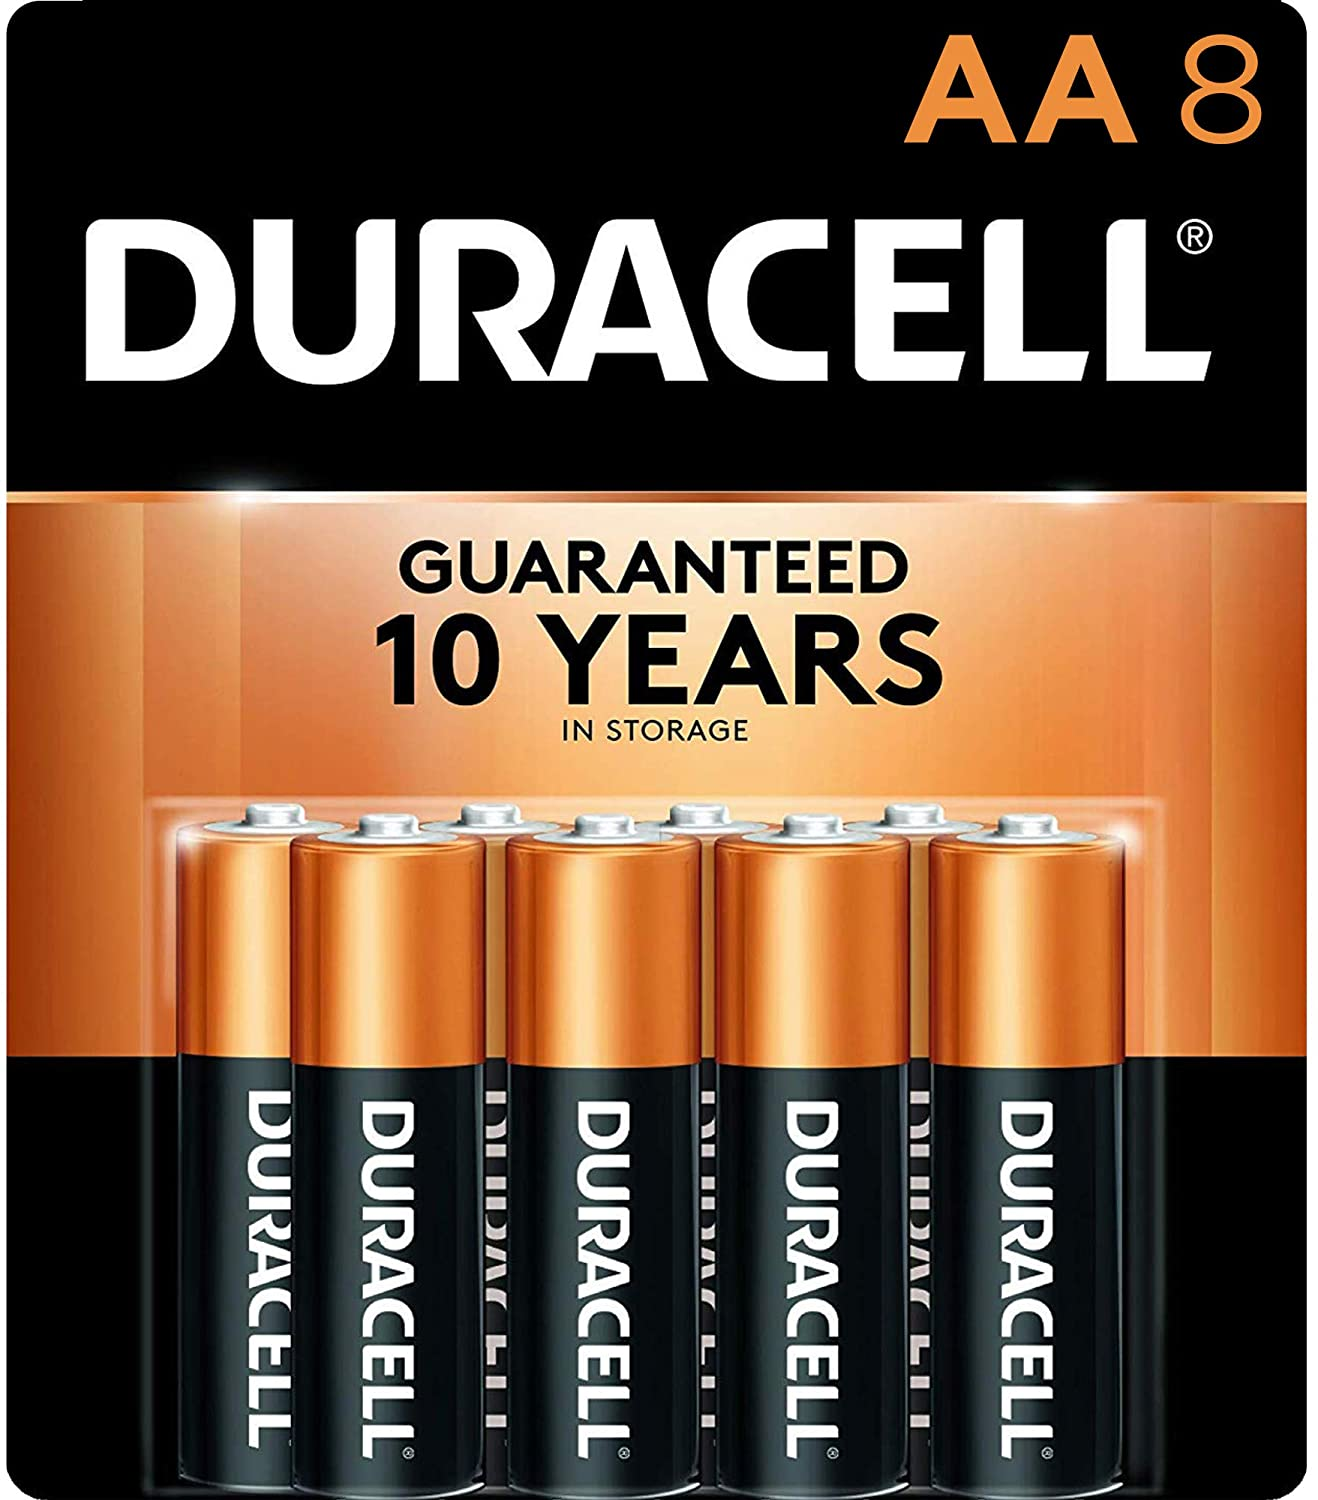
\includegraphics[scale=0.1]{aabatteries.jpg}

\begin{flushleft}
    A typical set of AA batteries by Duracell at 1.5 volts.
    \newline

    Online store link: \newline
    \footnotesize\url{https://www.amazon.com/Duracell-CopperTop-Batteries-all-purpose-household/dp/B003SI0TD4}

\end{flushleft}

\hypertarget{silica}{}
\subsubsection{Silica Gel}

\hspace{2em}
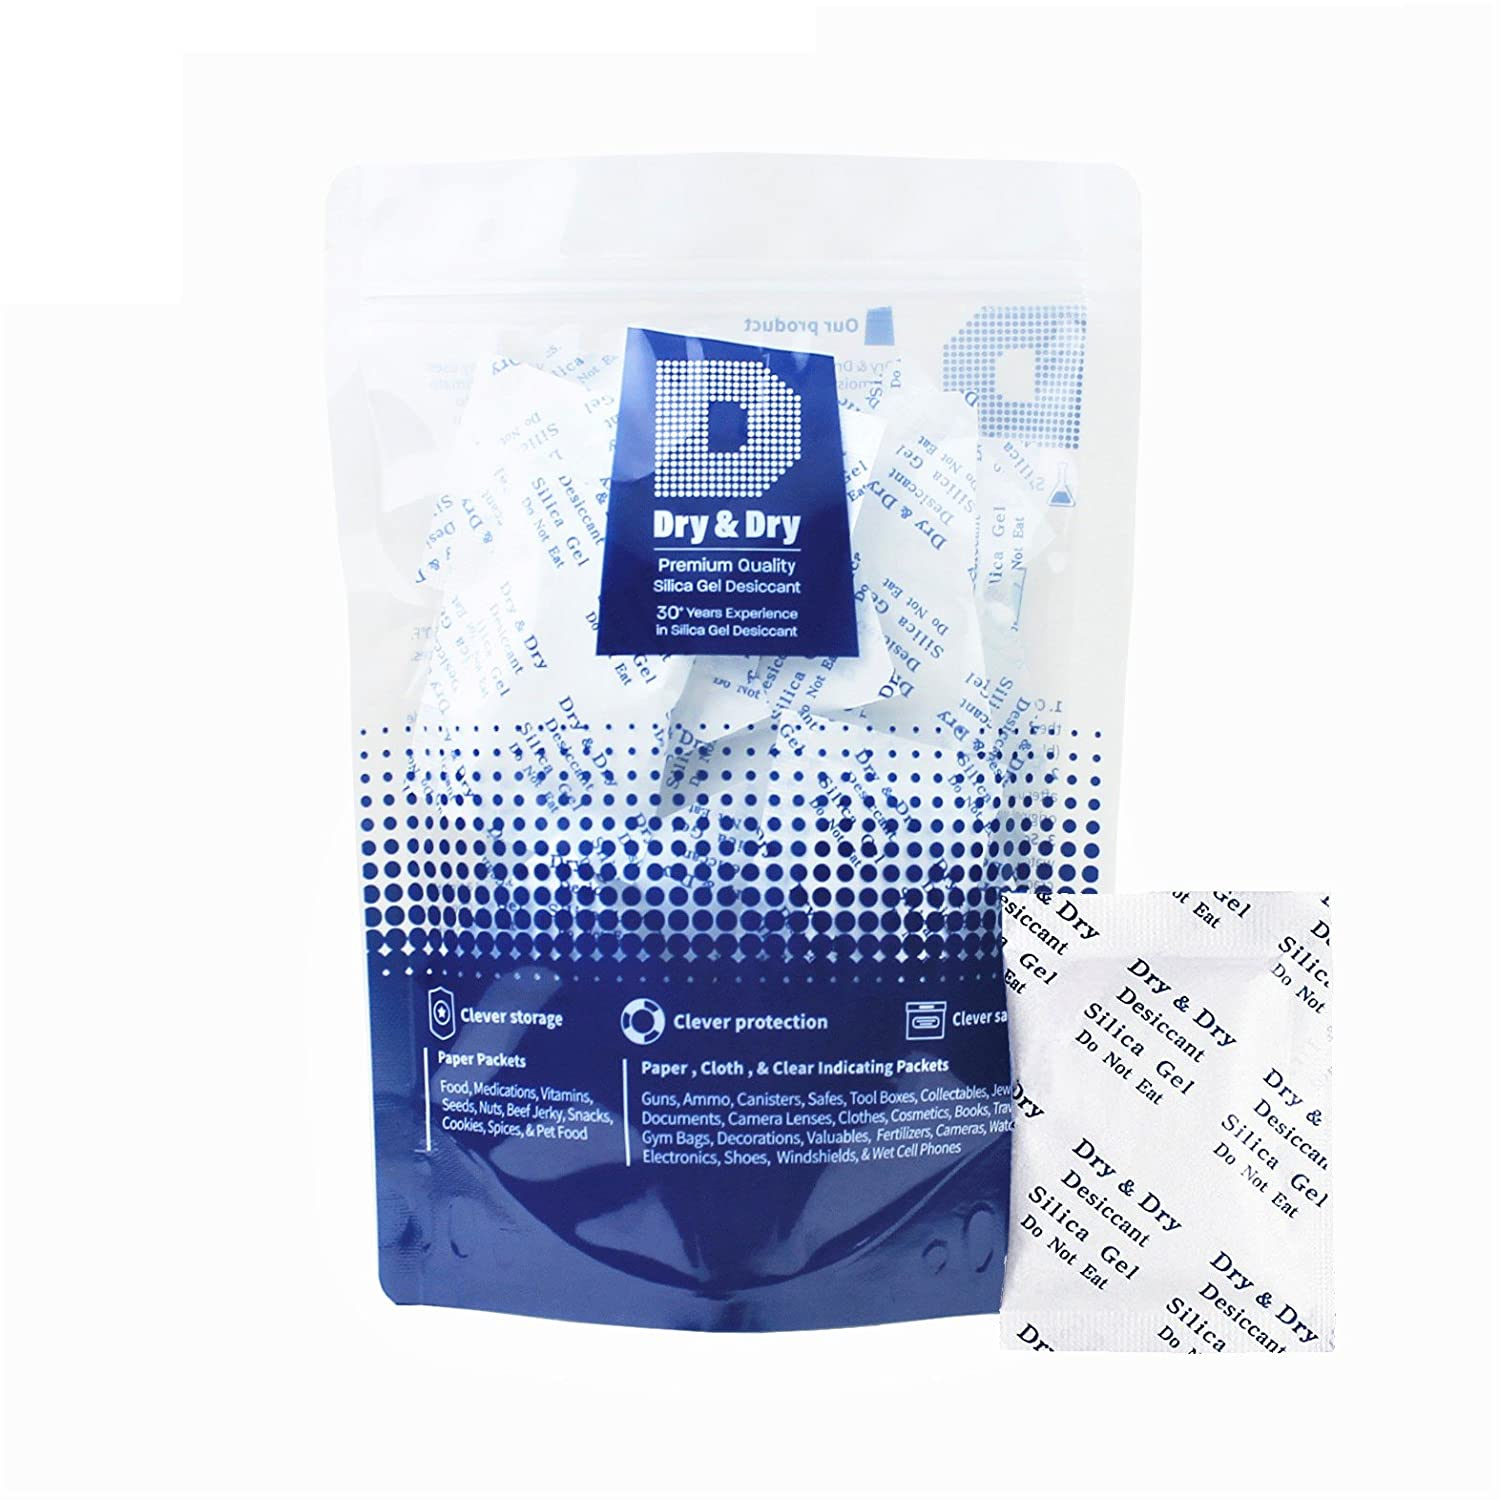
\includegraphics[scale=0.07]{silica.jpg}

\begin{flushleft}
    A packet of silica gels in the Nalgene bottle will be used as a dehumidifier, 
    to help maintain a humidity and moisture free enclosure of the electronic 
    components.
    \newline

    Online store link: \newline
    \footnotesize\url{https://www.amazon.com/Dry-Premium-Packets-Desiccant-Dehumidifiers/dp/B00DYKTS9C}

\end{flushleft}

\hypertarget{glue}{}
\subsubsection{Clear Silicone Sealant}

\hspace{2em}
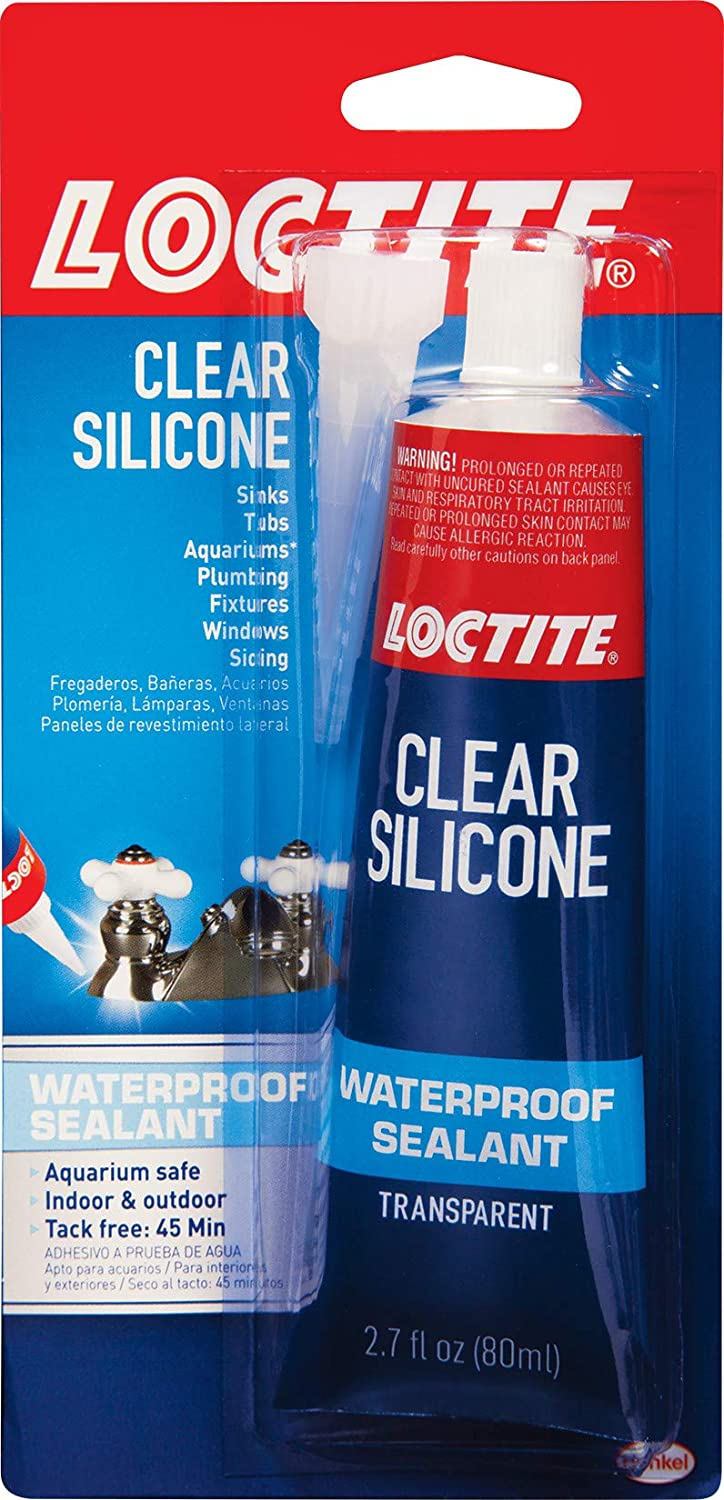
\includegraphics[scale=0.1]{silicone.jpg}

\begin{flushleft}
    A clear, waterproof silicone sealant to adhere and protect the exterior 
    sensors from water damage. It will also be used to adhere the jumper wires 
    in place and seal the two cables that will be protruding through the lid 
    of the Nalgene bottle.
    \newline

    Online store link: \newline
    \footnotesize\url{https://www.amazon.com/Loctite-Silicone-Waterproof-2-7-Ounce-908570/dp/B0002BBX3U}

\end{flushleft}


  % This document should describe the entire assembly of the device, NOTE: only some devices will be pre-soldered so include some form of table of contents to jump to if you're buoy is pre-soldered.
\section{Device Construction}

\subsection{Production Buoy}

\subsection{Prototype Buoy}

\begin{flushleft}
    The prototype instructions are to set up the user with a breadboard layout of the buoy in order to have a more 
    accessible format of making changes and updates to the design of the hardware buoy.
\end{flushleft}

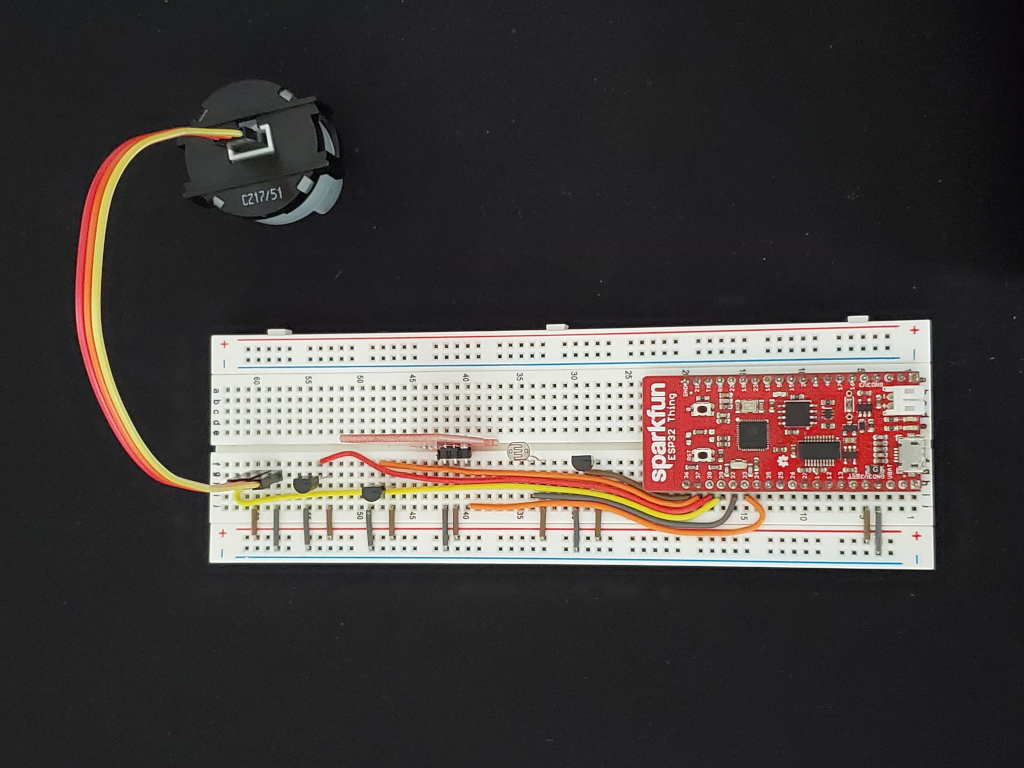
\includegraphics[scale=1]{buoy_breadboard.jpg}

\begin{enumerate}
    \item Place the Sparkfun ESP32 on the end of the breadboard and offset right from the center of the breadboard,
    so the left-side GPIO pins have more room to insert jumper wires. The pins on the Sparkfun should go in \textbf{Columns 1 through 20}, for the \textbf{Rows A and H}.
    \item Insert the jumper wires for the breadboard power rails, connecting the ESP32 pin \textbf{3V3} to the Positive rail and ESP32 pin \textbf{GND} to the Negative rail.
    \item Add the first temprature sensor to \textbf{Columns 28, 29, 30}, flat-side facing to the middle of the breadboard. Connect \textbf{Column 28 to Positive Rail} and \textbf{Column 30 to Negative Rail}. Connect \textbf{Column 29 to Column 20} which connects to ESP32 pin \textbf{36}.
    \item Add the photoresistor to \textbf{Columns 33, 34}, polarity does not matter. Connect \textbf{Column 33 to Positive Rail} and \textbf{Column 34 to Column 16} which connects ESP32 pin \textbf{32}.
    \item Add the salinty sensor to \textbf{Columns 40, 41, 42}, Power LED facing away from center of breadboard. Connect \textbf{Column 42 to Negative Rail}, \textbf{Column 41 to Positive Rail}, and \textbf{Column 40 to Column 15} which is ESP32 pin \textbf{33}.
    \item Add the second temprature sensor to \textbf{Columns 47, 48, 49}, flat-side facing to the middle of the breadboard. Connect \textbf{Column 47 to Positive Rail} and \textbf{Column 49 to Negative Rail}. Connect \textbf{Column 48 to Column 20} which connects to ESP32 pin \textbf{37}.
    \item Add the third temprature sensor to \textbf{Columns 53, 54, 55}, flat-side facing to the middle of the breadboard. Connect \textbf{Column 28 to Positive Rail} and \textbf{Column 30 to Negative Rail}. Connect \textbf{Column 29 to Column 20} which connects to ESP32 pin \textbf{38}.
    \item Add the insolation sensor (tab connector orientated up), where the \textbf{Left Pin is +5V}, \textbf{Center Pin is output}, and \textbf{Right Pin is GND} to \textbf{Columns 60, 59 , 58} respectively. Connect \textbf{Column 60 to Positive Rail}, \textbf{Column 58 to Negative Rail}, and \textbf{Column 59 to Column 17} which is ESP32 pin \textbf{39}.
\end{enumerate}
  % Describe the low-level communication protocols for all communications
\section{Communication Protocols}
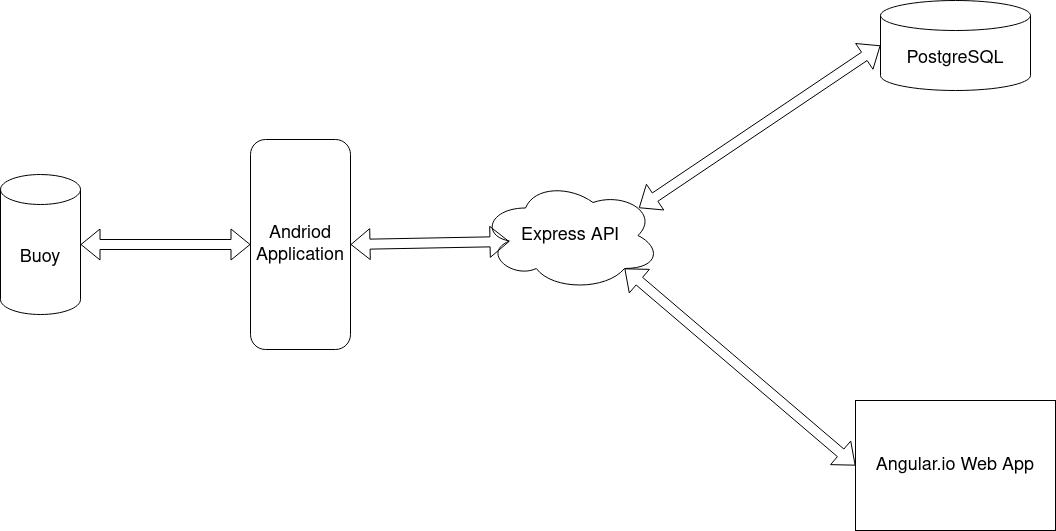
\includegraphics[scale=0.3]{wwxs.png}
\subsection{Web API Communication Protocol}
The goal of these API calls is to create, read, update and delete entries safley in the database. And to clearly communicate with the client (usually the web UI or the Mobile Application) the API must give meaningful responses. Any form of response designed to not return data will reply with JSON data with a message field. For example, a 200 "OK" response would return with this message in the body:
\begin{lstlisting}
  {
    message: "OK"
  }
\end{lstlisting}
In general, here are a list of create, read, update and delete calls and what they should return:
\begin{center}
  \begin{tabular}{| p{0.2\linewidth} | p{0.4\linewidth}  | p{0.4\linewidth} |}
    \hline
    HTTP Request Type & On success & On failure \\
    \hline
    GET "/" & 200 and all entries in the table & 400 Bad Request \\
    \hline
    GET "/:id" & 200 all entries in the table & 400 Bad Request \\
    & whose private key matches & 404 Not Found \\
    \hline
    POST "/" & 201 and the entry placed in the table & 400 Bad Request \\
    \hline
    PUT "/:id" & 200 and the entire entry updated & 400 Bad Request \\
    & with updated information & 404 Not Found \\
    \hline
    DELETE "/:id" & 200 OK & 400 Bad Request \\
    & & 404 Not Found \\
    \hline
  \end{tabular}
\end{center}
And the routes:
\begin{center}
  \begin{tabular}{| p{0.2\linewidth} | p{0.4\linewidth}  | p{0.4\linewidth} |}
    \hline
    Route & Description & Supported Methods \\
    \hline
    /buoy & Information associated with every buoy. & GET, GET + /:id, POST, PUT, DELETE + /:id \\
    \hline
    /data & Information associated with data pointed collected by buoys. & GET, GET + /:id, POST \\
    \hline
    /group & Information associated with groups of users. & GET, GET + /:id, POST, PUT, DELETE + /:id \\
    \hline
    /session & \emph{Deprecated} Information associated with user sessions. & \emph{Deprecated} \\
    \hline
    /user & Information associated with users and login. & GET, GET + /:id, POST \\
    \hline
    /user/login & Returns web token for authorization. & POST \\
    \hline
  \end{tabular}
\end{center}
\subsubsection{Buoy}
\texttt{
\{ \\
    "id": identification number (int)\\
    "name": meaningful buoy name (string)\\
    "mac": mac/hardware address of buoy (string)\\
    "pubKey": public key to encrypt information for buoy (string)\\
    "lastRetrieval": last date the buoy submitted data (sql date)\\
    "version": version of buoy (string)\\
    "createdAt": creation date (sql date)\\
    "updatedAt": updated date (sql date)\\
    "groupId": identification number the group the buoy belongs too (integer, foriegn key)\\
\}
}
\subsubsection{Data}
\texttt{
\{ \\
    "id": identification number (int) \\
    "updatedAt": updated date (sql date) \\
    "createdAt": creation date (sql date) \\
    "timestamp": collection timestamp (sql date) \\
    "surfTemp": surface temprature collected within the buoy (float) \\
    "surfInsolation": measure of sunlight exposure in the buoy (float) \\
    "shallowSalinity": measure of salinity at 2' depth (float) \\
    "shallowTemp": measure of water temprature at 2' depth (float) \\
    "depthTemp": measure of water temprature at 7' depth (float) \\
    "depthTurbidity": measure of sunlight at 7' depth (float) \\
    "buoyId": id of buoy that collected the data (int, foreign key) \\
    "userId": id of user that collected the data (int, foreign key) \\
\}
}
\subsubsection{Group}
\texttt{
\{ \\
    "id": identification number (int) \\
    "name": meaningful group name (string) \\
    "updatedAt": updated date (sql date) \\
    "createdAt": creation date (sql date) \\
\}
}
\subsubsection{User}
\texttt{
\{ \\
    "id": identification number (int) \\
    "updatedAt": updated date (sql date) \\
    "createdAt": creation date (sql date) \\
    "username": meaningful username (string) \\
    "password": meaninful password (string) \\
    "email": user's email (string) \\
    "role":  user's role (string) \\
    "lastLogin": last login date (sql date) \\
    "groupId": identification number the group the user belongs to (integer, foriegn key) \\
    "token": string formatted JSON web token (string) \\
\}
}
% make a 1;1 list of every route and method in the node.js api

\end{document}
